\chapter{Wykorzystane narzędzia}

\section{Język Python}
Język Python jest jednym z najpopularniejszych języków wykorzystywanych do analizy danych oraz uczenia maszynowego. Z resztą jest on ogólnie jednym z najpopularniejszych języków, co jest potwierdzone przez badanie \bibtitle{2023 Developer Survey} \cite{stackoverflow-survey} przeprowadzanie przez Stack Overflow, gdzie uplasował się na 4 miejscu w rankingu najpopularniejszych.

Został on wykorzystany ze względu na ogromną liczbę bibliotek, które są do niego dostępne. Kilka spośród nich, które odegrały kluczową rolę podczas realizacji niniejszego tematu, zostały opisane w poniższych sekcjach. Ponadto umożliwia on bardzo szybkie prototypowanie i eksperymentowanie, co również zostało docenione. Jest to bowiem język wysokopoziomowy i zwalnia programistów z zajmowania się wieloma kwestiami. Jest elastyczny ze względu na swoje wieloparadygmatowe podejście: obiektowe, proceduralne jak i funkcyjne. Ostatecznie jest językiem skryptowym i brak narzutu czasowego na kompilację znacznie skraca pętle zwrotną między pisaniem kodu, a oglądaniem jego skutków.

\subsection{Biblioteki SpaCy i Stanza}
Biblioteki \code{SpaCy} i \code{Stanza} to popularne dla języka Python drogi do przeprowadzenia analizy tekstów w języku naturalnym. Zostały przedstawione razem, ponieważ różnice między nimi są niewielkie i za pomocą obu można realizować niemal identyczne cele. O wykorzystaniu pierwszej lub drugiej zadecydowały mało istotne szczegóły, takie jak interfejs, który w danym momencie wydawał się wygodniejszy. Z powodzeniem można by było jednak ograniczyć się do wykorzystania jednej z nich.

Obie z przytoczonych bibliotek pozwalają na analizę tekstów w różnych językach, w tym w języku polskim. Pozwalają na przeprowadzenie tokenizacji, czyli podziału tekstów na poszczególne słowa oraz lematyzacji, czyli zamiany każdego słowa na jego bazową formę. Można za ich pomocą także znaleźć w tekście wszystkie nazwy własne poprzez analizę NER (Named Entity Recognition), czy przypisać dla każdeog słowa nazwę części mowy, którą stanowi. 

\subsection{Biblioteka sqlparse}
Biblioteka \code{sqlparse} nie jest wyjątkowo rozbudowana pod względem oferowanych funkcji, lecz jej niezaprzeczalna popularność potwierdza, że doskonale wpasowała się w potrzeby deweloperów. Tak jak mówi nazwa, \code{sqlparse} pozwala na parsowanie zapytań SQL. Sprowadza się to do konwersji podanego jako wejście zapytania na poszczególne tokeny, takie jak słowa kluczowe \code{SELECT}, \code{WHERE}, nazwy kolumn i tabel oraz wartości. Każdy z wyprodukowanych przy tym tokenów posiada typ, mówiący co sobą reprezentuję. Zauważono jednak, że biblioteka ta nie jest bezbłędna i w szczególności dla złożonych zapytań może się mylić, więc należy mieć to na uwadze podczas jej wykorzystywania.

\subsection{Biblioteka sqlglot}
Biblioteka \code{sqlglot} to naprawdę rozbudowane i wszechstronne narzędzie służące do pracy z instrukcjami SQL. Wspiera ponad 20 różnych dialektów i pozwala na transpilację, czyli konwersję instrukcji SQL pomiędzy nimi. Ponadto zapewnia szczegółową walidację i formatowanie. Wśród jej bardziej zaawansowanych funkcji znajduję się optymalizacja zapytań, a nawet symulowanie całego silnika bazodanowego, co pozwala na rzeczywiste wykonywanie instrukcji.

Najbardziej pożądaną podczas realizacji niniejszej pracy funkcją okazało się parsowanie zapytań do drzew \code{AST} (ang. Abstract Syntax Tree) i dalszej pracy z nimi. Są to struktury, które pozwalają na reprezentację programów, czy też instrukcji w dowolnym języku formalnym w wygodnej do analizy i modyfikacji postaci. Drzewo \code{AST} dla przykładowego zapytania SQL zostało przedstawione na rysunku \ref{fig:sql-ast-example}.

\begin{figure}[ht!]
  \centering
  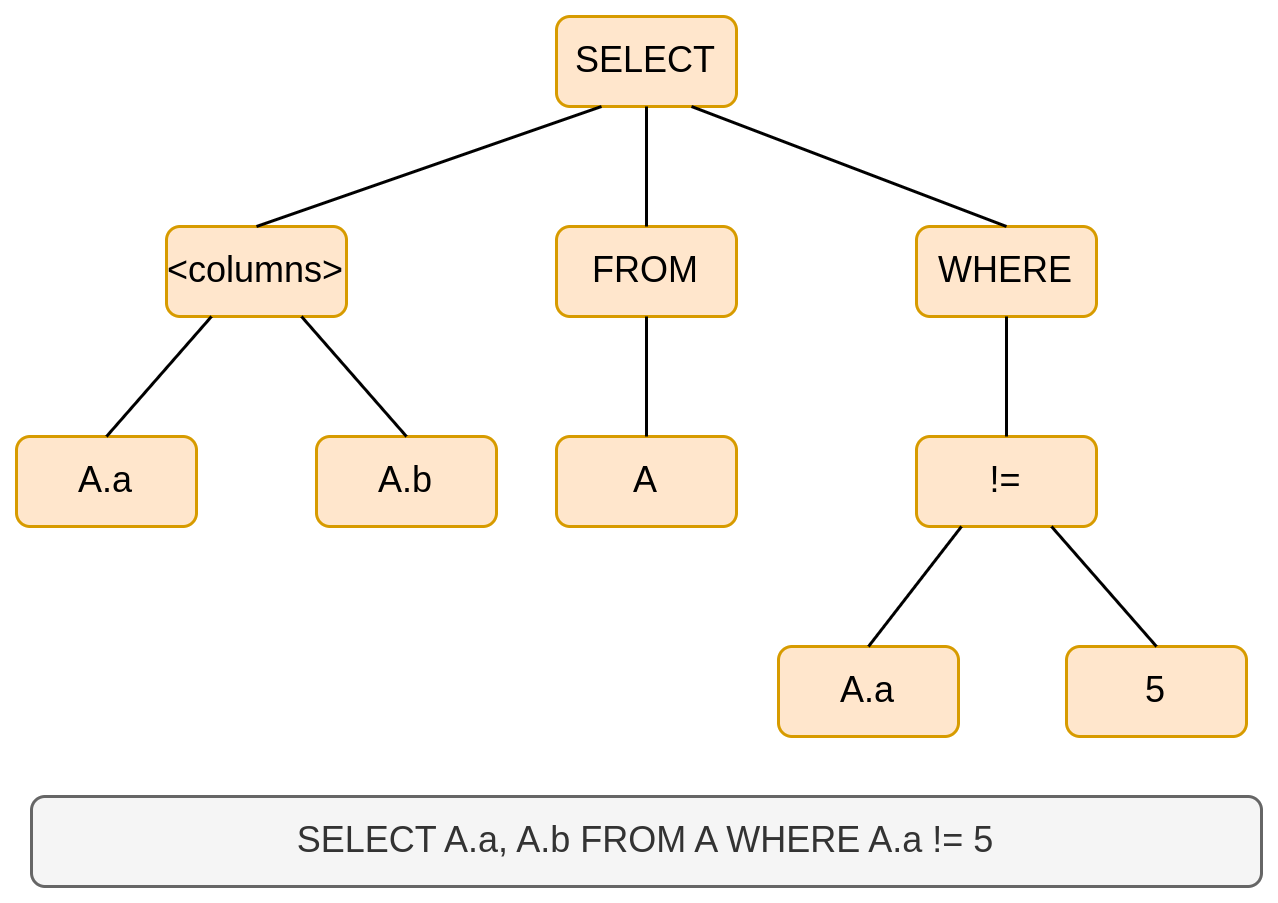
\includegraphics[width=0.55\linewidth]{images/ast_example.png}
  \caption{Drzewo AST dla przykładowego zapytania SQL}
  \label{fig:sql-ast-example}
\end{figure}

\section{Visual Studio Code}
Visual Studio Code to wszechstronny edytor stworzony przez Microsoft. Zgodnie z tegoroczną ankietą \bibtitle{2023 Developer Survey} \cite{stackoverflow-survey} przeprowadzoną przez Stack Overflow jest on najczęściej wybieranym przez deweloperów środowiskiem programistycznym. Tym co je wyróżnia jest prostota przy jednoczesnej potędze płynącej z niespotykanej elastyczności. Dostępna jest bowiem ogromna liczba łatwych w instalacji rozszerzeń. Pozwalają one dostosować to środowisko niemal do każdego możliwego scenariusza wykorzystania.

Podczas realizacji pracy szczególnie użyteczne okazały się rozszerzenia dla języka Python dodające kolorowanie składni, dokończanie kodu, debugowanie, czy też wsparcie dla interaktywnych notesów Jupyter. Poza tym intensywnie wykorzystywane było rozszerzenie do pracy z narzędziem Docker. Jeśli chodzi o podstawowe funkcje środowiska to bardzo użyteczna okazała się integracja z systemem kontroli wersji oraz zaawansowane wyszukiwanie i zastępowanie.

\section{Docker}
Docker to bardzo potężne i powszechnie wykorzystywane narzędzie na którym opiera się znaczna część funkcjonującego oprogramowania. Umożliwia on tworzenie, zarządzanie i uruchamianie aplikacji w izolowanych kontenerach. Pozwalają one deweloperom na zapakowanie aplikacji z zależnościami i środowiskiem uruchomieniowym, co zapewnia spójność działania na różnych platformach.

Podczas realizacji niniejszego projektu Docker okazał się szczególnie użyteczny w kontekście uruchamiania istniejących modeli uczenia maszynowego. Część z nich była od razu gotowa do działania w kontenerze, a inne zostały przystosowane. Okres czasu w którym te rozwiązania powstawały jest bowiem bardzo rozległy, więc zależności z których korzystają znacznie się różnią i trudno jest je ze sobą pogodzić. W przypadku różnic jedynie w pakietach języka Python możliwe by było skorzystanie ze znacznie prostszego narzędzia \code{conda}, lecz poziom izolacji tworzonych za jego pomocą środowisk jest znacznie ograniczony i jak się okazało niewystarczający.

\begin{comment}
Inne narzędzia:
- git
- conda
\end{comment}